\documentclass[11pt,a4paper,twoside]{epig}
\usepackage[latin1]{inputenc}
\usepackage{times}
\usepackage{helvet}
%package pour les algo
\usepackage{algorithm}
\usepackage{algorithmic}
\usepackage{comment}

\pagestyle{empty}
\newcommand{\smallitem}{\vspace*{-2mm}\item}
\renewcommand{\baselinestretch}{0.95}
\marginparwidth 0pt 
\evensidemargin 2.2cm 
\oddsidemargin 1.8cm 
\topmargin 0cm 
\textwidth 12cm 
\textheight 19cm

\makeatletter
\renewcommand{\fnum@figure}{\textbf{\fontsize{10}{10}\selectfont\sffamily\figurename~\thefigure}}
\renewcommand{\fnum@table}{\textbf{\fontsize{10}{10}\selectfont\sffamily\tablename~\thetable}}
\makeatother


\newcommand{\auteur}[1]{
	\begin{center}
	{#1}
	\end{center}
}

\newcommand{\titre}[1]{
	\begin{center}
	{\large\bfseries \sffamily {#1}}
	\end{center}
}

\newcommand{\affiliation}[1]{
	\noindent
	{\small{#1}}
}


\usepackage{hyperref}
\usepackage{amsmath}  % Maths
\usepackage{amsfonts} % Maths
\usepackage{amssymb}  % Maths
\usepackage{stmaryrd} % Maths (crochets doubles)

\usepackage{url}     % Mise en forme + liens pour URLs
\usepackage{array}   % Tableaux évolués

\usepackage{prettyref}
\newrefformat{def}{Def.~\ref{#1}}
\newrefformat{fig}{Fig.~\ref{#1}}
\newrefformat{pro}{Property~\ref{#1}}
\newrefformat{pps}{Proposition~\ref{#1}}
\newrefformat{lem}{Lemma~\ref{#1}}
\newrefformat{thm}{Theorem~\ref{#1}}
\newrefformat{sec}{Sect.~\ref{#1}}
\newrefformat{ssec}{Subsect.~\ref{#1}}
\newrefformat{suppl}{Appendix~\ref{#1}}
\newrefformat{eq}{Eq.~\eqref{#1}}
\def\pref{\prettyref}

\usepackage{ntheorem}
\theoremheaderfont{\fontsize{10}{10}\sffamily\bfseries}
%\newtheorem*{example}{Example}{\itshape}{}
\newtheorem{example}{Example}{\itshape}{}
\newtheorem{definition}{Definition}{\itshape}{}

\usepackage{tikz}
\newdimen\pgfex
\newdimen\pgfem
\usetikzlibrary{arrows,shapes}
%\usetikzlibrary{shadows,scopes}
%\usetikzlibrary{positioning}
%\usetikzlibrary{matrix}
%\usetikzlibrary{decorations.text}
%\usetikzlibrary{decorations.pathmorphing}



%\input{macros/macros}

% Macros générales
\def\Pint{\textsc{PINT}}

% Notations générales pour PH
\newcommand{\PH}{\mathcal{PH}}
\newcommand{\PHs}{\Sigma}
\newcommand{\PHl}{L}
\newcommand{\PHp}{\textcolor{red}{\mathcal{P}}}
\newcommand{\PHproc}{\mathcal{P}}
\newcommand{\PHa}{\PHh}
\newcommand{\PHh}{\mathcal{H}}
\newcommand{\PHn}{\mathcal{N}}

\newcommand{\PHhitter}{\mathsf{hitter}}
\newcommand{\PHtarget}{\mathsf{target}}
\newcommand{\PHbounce}{\mathsf{bounce}}
\newcommand{\PHsort}{\Sigma}

\def\f#1{\mathsf{#1}}
\def\focals{\f{focals}}
\def\play{\cdot}
\def\configs#1{\mathbb C_{#1\rightarrow a}}

\newcommand{\PHfrappeA}{\rightarrow}
\newcommand{\PHfrappeB}{\Rsh}
\newcommand{\PHfrappe}[3]{#1\PHfrappeA#2\PHfrappeB#3}
\newcommand{\PHfrappebond}[2]{#1\PHfrappeB#2}
\newcommand{\PHobjectif}[2]{\mbox{$#1\PHfrappeB^*\!#2$}}
\newcommand{\PHconcat}{::}
\newcommand{\PHneutralise}{\rtimes}

\def\PHget#1#2{{#1[#2]}}
\newcommand{\PHchange}[2]{(#1 \Lleftarrow #2)}
\newcommand{\PHarcn}[2]{\mbox{$#1\PHneutralise#2$}}
\newcommand{\PHjoue}{\cdot}

\newcommand{\PHetat}[1]{\mbox{$\langle #1 \rangle$}}

% Notations spécifiques à ce papier
\newcommand{\PHdirectpredec}[1]{\PHs^{-1}(#1)}
\newcommand{\PHpredec}[1]{\f{pred}(#1)}
\newcommand{\PHpredecgene}[1]{\f{reg}({#1})}
\newcommand{\PHpredeccs}[1]{\PHpredec{#1} \setminus \Gamma}

\newcommand{\PHincl}[2]{#1 :: #2}

\def\ctx{\varsigma}
\def\ctxOverride{\Cap}
\def\PHstate#1{\langle #1 \rangle}

\def\DEF{\stackrel{\Delta}=}
\def\EQDEF{\stackrel{\Delta}\Leftrightarrow}

\def\intervalless{<_{[]}}

%\input{macros/macros-ph}

% Notations pour le modèle de Thomas (depuis thèse)
\newcommand{\GRN}{\mathcal{GRN}}
\newcommand{\IG}{\mathcal{G}}
\newcommand{\GRNreg}[1]{\Gamma^{-1}(#1)}
\newcommand{\GRNres}[2]{\mathsf{Res}_{#1}(#2)}
\newcommand{\GRNallres}[1]{\mathsf{Res}_{#1}}
\newcommand{\GRNget}[2]{\PHget{#1}{#2}}
\newcommand{\GRNetat}[1]{\PHetat{#1}}

\def\levels{\mathsf{levels}}
\def\levelsA#1#2{\levels_+(#1\rightarrow #2)}
\def\levelsI#1#2{\levels_-(#1\rightarrow #2)}

\newcommand{\Kinconnu}{\emptyset}
\newcommand{\RRGva}[3]{#1 \stackrel{#2}{\longrightarrow} #3}
\newcommand{\RRGgi}{\mathcal{G}}
\newcommand{\RRGreg}[1]{\RRGgi_{#1}}

\tikzstyle{grn}=[every node/.style={circle,draw=black,outer sep=2pt,minimum
                size=15pt,text=black}, node distance=1.5cm]
\tikzstyle{act}=[->,draw=black,thick,color=black]
\tikzstyle{inh}=[>=|,-|,draw=black,thick, text=black,label]
\tikzstyle{inf}=[->,draw=colorinf,thick,color=colorinf]
\tikzstyle{elabel}=[fill=none,text=black, above=-2pt,%sloped,
minimum size=10pt, outer sep=0, font=\scriptsize, draw=none]
\tikzstyle{sg}=[every node/.style={outer sep=2pt,minimum
                size=15pt,text=black}, node distance=2cm]

%\input{macros/macros-grn}

\usepackage{ifthen}
%\usepackage{tikz}
%\usetikzlibrary{arrows,shapes}

\definecolor{lightgray}{rgb}{0.8,0.8,0.8}
\definecolor{lightgrey}{rgb}{0.8,0.8,0.8}

\tikzstyle{boxed ph}=[]
\tikzstyle{sort}=[fill=lightgray,rounded corners]
\tikzstyle{process}=[circle,draw,minimum size=15pt,fill=white,
font=\footnotesize,inner sep=1pt]
\tikzstyle{black process}=[process, fill=black,text=white, font=\bfseries]
\tikzstyle{gray process}=[process, draw=black, fill=lightgray]
\tikzstyle{current process}=[process, draw=black, fill=lightgray]
\tikzstyle{process box}=[white,draw=black,rounded corners]
\tikzstyle{tick label}=[font=\footnotesize]
\tikzstyle{tick}=[black,-]%,densely dotted]
\tikzstyle{hit}=[->,>=angle 45]
\tikzstyle{selfhit}=[min distance=30pt,curve to]
\tikzstyle{bounce}=[densely dotted,->,>=latex]
\tikzstyle{hl}=[font=\bfseries,very thick]
\tikzstyle{hl2}=[hl]
\tikzstyle{nohl}=[font=\normalfont,thin]

\newcommand{\currentScope}{}
\newcommand{\currentSort}{}
\newcommand{\currentSortLabel}{}
\newcommand{\currentAlign}{}
\newcommand{\currentSize}{}

\newcounter{la}
\newcommand{\TSetSortLabel}[2]{
  \expandafter\repcommand\expandafter{\csname TUserSort@#1\endcsname}{#2}
}
\newcommand{\TSort}[4]{
  \renewcommand{\currentScope}{#1}
  \renewcommand{\currentSort}{#2}
  \renewcommand{\currentSize}{#3}
  \renewcommand{\currentAlign}{#4}
  \ifcsname TUserSort@\currentSort\endcsname
    \renewcommand{\currentSortLabel}{\csname TUserSort@\currentSort\endcsname}
  \else
    \renewcommand{\currentSortLabel}{\currentSort}
  \fi
  \begin{scope}[shift={\currentScope}]
  \ifthenelse{\equal{\currentAlign}{l}}{
    \filldraw[process box] (-0.5,-0.5) rectangle (0.5,\currentSize-0.5);
    \node[sort] at (-0.2,\currentSize-0.4) {\currentSortLabel};
   }{\ifthenelse{\equal{\currentAlign}{r}}{
     \filldraw[process box] (-0.5,-0.5) rectangle (0.5,\currentSize-0.5);
     \node[sort] at (0.2,\currentSize-0.4) {\currentSortLabel};
   }{
    \filldraw[process box] (-0.5,-0.5) rectangle (\currentSize-0.5,0.5);
    \ifthenelse{\equal{\currentAlign}{t}}{
      \node[sort,anchor=east] at (-0.3,0.2) {\currentSortLabel};
    }{
      \node[sort] at (-0.6,-0.2) {\currentSortLabel};
    }
   }}
  \setcounter{la}{\currentSize}
  \addtocounter{la}{-1}
  \foreach \i in {0,...,\value{la}} {
    \TProc{\i}
  }
  \end{scope}
}

\newcommand{\TTickProc}[2]{ % pos, label
  \ifthenelse{\equal{\currentAlign}{l}}{
    \draw[tick] (-0.6,#1) -- (-0.4,#1);
    \node[tick label, anchor=east] at (-0.55,#1) {#2};
   }{\ifthenelse{\equal{\currentAlign}{r}}{
    \draw[tick] (0.6,#1) -- (0.4,#1);
    \node[tick label, anchor=west] at (0.55,#1) {#2};
   }{
    \ifthenelse{\equal{\currentAlign}{t}}{
      \draw[tick] (#1,0.6) -- (#1,0.4);
      \node[tick label, anchor=south] at (#1,0.55) {#2};
    }{
      \draw[tick] (#1,-0.6) -- (#1,-0.4);
      \node[tick label, anchor=north] at (#1,-0.55) {#2};
    }
   }}
}
\newcommand{\TSetTick}[3]{
  \expandafter\repcommand\expandafter{\csname TUserTick@#1_#2\endcsname}{#3}
}

\newcommand{\myProc}[3]{
  \ifcsname TUserTick@\currentSort_#1\endcsname
    \TTickProc{#1}{\csname TUserTick@\currentSort_#1\endcsname}
  \else
    \TTickProc{#1}{#1}
  \fi
  \ifthenelse{\equal{\currentAlign}{l}\or\equal{\currentAlign}{r}}{
    \node[#2] (\currentSort_#1) at (0,#1) {#3};
  }{
    \node[#2] (\currentSort_#1) at (#1,0) {#3};
  }
}
\newcommand{\TSetProcStyle}[2]{
  \expandafter\repcommand\expandafter{\csname TUserProcStyle@#1\endcsname}{#2}
}
\newcommand{\TProc}[1]{
  \ifcsname TUserProcStyle@\currentSort_#1\endcsname
    \myProc{#1}{\csname TUserProcStyle@\currentSort_#1\endcsname}{}
  \else
    \myProc{#1}{process}{}
  \fi
}

\newcommand{\repcommand}[2]{
  \providecommand{#1}{#2}
  \renewcommand{#1}{#2}
}
\newcommand{\THit}[5]{
  \path[hit] (#1) edge[#2] (#3#4);
  \expandafter\repcommand\expandafter{\csname TBounce@#3@#5\endcsname}{#4}
}
\newcommand{\TBounce}[4]{
  (#1\csname TBounce@#1@#3\endcsname) edge[#2] (#3#4)
}

\newcommand{\TState}[1]{
  \foreach \proc in {#1} {
    \node[current process] (\proc) at (\proc.center) {};
  }
}



\hyphenpenalty 1000

\newcommand{\FIG}[4]
{\begin{figure}[!hbt]
\begin{center}
\rotatebox{270}{\includegraphics[width=#1]{#2}}
\caption{\label{fig:#3}#4\vspace{-5mm}}
\end{center}
\end{figure}}



\begin{document}

\titre{Integrating time-series data on large-scale cell-based models: application to skin differentiation}
\auteur{Louis Fippo Fitime$^1$, Andrea Beica$^1$, Olivier Roux$^1$ and Carito Guziolowski$^{1}$}
\affiliation{$^1 $
LUNAM Universit\'e, \'Ecole Centrale de Nantes, IRCCyN UMR CNRS 6597\\
(Institut de Recherche en Communications et Cybern\'etique de Nantes)\\
1 rue de la No\"e -- B.P. 92101 -- 44321 Nantes Cedex 3, France.\\
\texttt{Louis.Fippo-Fitime@irccyn.ec-nantes.fr}}
\\

\section*{Abstract}
\vspace{-2mm}
The way living organisms work and develop themselves is controlled by large and complex 
networks of genes, proteins, small molecules, and their interactions, \textbf{called} biological 
regulatory networks. Confronting time-series gene expression data with models may allow us to
examine and characterize the dynamics of elements that compose \textbf{such  regulatory networks}. 
In this work, we propose a way to model and simulate large-scale regulatory networks, by using the 
Process Hitting (PH) framework, in order to verify if the model \textbf{can predict} the experimental measures.
The preliminary work presented here proposes: (1) a semi-automatic method to build a PH from
a regulatory network of biochemical reactions, (2) a discretization scheme of the continuous time-series measurements, 
and (3) an approach to estimate the PH stochastic simulation parameters in an unbiased manner.
\vspace{-2mm}



\section{Introduction}
The comprehension of the mechanisms involved in the regulation of a \textbf{living cell} is a fundamental 
issue. These mechanisms can be modeled as \textbf{biological} regulatory networks, which analysis requires to preliminary build a 
mathematical or computational model. 
By just considering qualitative regulatory effects between components, biological regulatory networks
depict fairly well biological systems, and can be built upon public repositories such as the Pathways 
Interaction Database \cite{schaefer2009pid}, and 
hiPathDB\cite{yu2012hipathdb} for human regulatory knowledge.


This work aims to propose a dynamical model of large-scale systems based on the formal integration 
(complete validation/invalidation) of high-throughput experimental time-series data.  So far this 
idea has been addressed separately by approaches that either: (a) focus first on
modeling at small-scale the system and then on refining or improving it through the fitting with
some data points, such as methods based on differential equations \cite{tyson2003sniffers,batt2005validation,mobashir2012simulated}, (b) integrate in an efficient and complete fashion large-scale models
and high-throughput data \textbf{regardless of the} system dynamics 
\cite{guziolowski2013exhaustively,mitsos2009identifying}, or 
(c) fit dynamical data to middle-scale networks using stochastic approaches, and
therefore without guarantee on finding global optima \cite{macnamara2012state}. Therefore, with this
work we intend to fill the gaps between the previously cited methodologies and converge to a more
realistic model of biological behavior.

For modeling and analyzing the biological system we rely on the Process Hitting (PH) framework\cite{PMR10-TCSB}, 
since it is especially useful for studying systems composed of biochemical interactions, and provides
stochastic simulation as well as efficient static methods to model dynamical properties of the system.
The PH framework uses qualitative and discrete information of the system, without requiring enormous parameter estimation tasks
 for its stochastic simulation. 
So far, this method has been successfully demonstrated only on very well-known systems and without exploiting 
high-throughput measures. We believe, however, that the use of high-throughput data has become unavoidable with 
the advent of massive, publicly available data sets in the form of well-standardized DNA microarray data and, 
more recently, in the form of phospho-proteomics data.  

The main methodological and preliminar results of this work are: (i) semi-automatic PH generation 
from a biological system composed of biochemical reactions, extracted from public databases;
(ii) discretization approach of time-series expression data, so we can 
reproduce these traces by using in a first attempt the PH stochastic simulation, and afterwards 
perform static reachability analyses to satisfy \textbf{these} data; and (iii) estimation of the the temporal and stochastic
parameters of the simulation, based on statistical analyses of the full-compendium of time-series expression data.
The biological system used as a case-study for this work is a cell-based model of skin differentiation, which 
is of key importance in  wound healing. 



\vspace{3mm}
\noindent

\section{Methods and data}
\subsection{The Process  Hitting Framework}
\label{ssec:PH}

%We present here the Process Hitting framework \cite{PMR10-TCSB} which will enable us to model 
%biological network.

%\vspace{3mm}

Process Hitting (PH) gathers a finite number of concurrent processes grouped into a finite set of sorts.
A sort stands for a component of a biological system while a process, which belongs to a unique sort, stands
for one of its expression levels. At any time, exactly one process of each sort is present. A state of the 
PH corresponds to such a set of processes. We denote here a process by $a_i$ where $a$ 
is the sort and $i$ is the process identifier within the sort $a$.
The concurrent interactions between processes are defined by a set of \emph{actions}.
Actions describe the replacement of a process by another of the same sort conditioned by the presence 
of at most one other process in the current state. An action is denoted by $\PHfrappe{a_i}{b_j}{b_k}$, 
which is read as ``$a_i$ \emph{hits} $b_j$ to make it bounce to $b_k$'', where $a_i,b_j,b_k$ are 
processes of sorts $a$ and $b$, called respectively \emph{hitter}, \emph{target} and \emph{bounce} of 
the action.

\begin{definition}[Process Hitting]\label{def:PH}
A \emph{Process Hitting} is a triple $(\PHs,\PHl,\PHa)$, where:
\begin{itemize}
\item $\PHs = \{a,b,\dots\}$ is the finite set of \emph{sorts};
\item $\PHl = \prod_{a\in\PHs} \PHl_a$ is the set of states with $\PHl_a = \{a_0,\dots,a_{l_a}\}$
the finite set of \emph{processes} of sort $a\in\Sigma$ and $l_a$ a positive integer, with $a\neq b\Rightarrow \PHl_a \cap \PHl_b = \emptyset$;
\item $\PHa = \{ \PHfrappe{a_i}{b_j}{b_k} \in \PHl_a \times \PHl_b \times \PHl_b \mid (a,b) \in \PHs^2
  \wedge b_j\neq b_k \wedge a=b\Rightarrow a_i=b_j\}$ is the finite set of \emph{actions}.
\end{itemize}
\end{definition}

\noindent
Given a state $s\in \PHl$, the process of sort $a\in\PHs$ present in $s$ is denoted by $\PHget{s}{a}$.
An action $h=\PHfrappe{a_i}{b_j}{b_k} \in \PHa$ is \emph{playable} in $s \in L$ if and only if $\PHget{s}{a}=a_i$ and $\PHget{s}{b} = b_j$.
In such a case, $(s\play h)$ stands for the state resulting from the play of the action $h$ in $s$, with
$\PHget{(s\play h)}{b} = b_k$ and $\forall c \in \PHs, c \neq b, \PHget{(s\play h)}{c} = \PHget{s}{c}$.

\paragraph{Modeling cooperation.}

As described in \cite{PMR10-TCSB}, the cooperation between processes to make another process bounce can be
expressed in PH by building a \emph{cooperative sort}.
\pref{fig:runningPH} shows an example of a cooperative sort $ab$ between sorts $a$ and $b$,
defined with 4 processes (one for each sub-state of the presence of processes $a_1$ and $b_1$).
For the sake of clarity, processes of $ab$ are indexed using the sub-state they represent.
Hence, $ab_{01}$ represents the sub-state $\PHstate{a_0,b_1}$, and so on.
Each process of sort $a$ and $b$ hit $ab$, which makes it bounce to the process reflecting the status of the sorts $a$
and $b$ (e.g., $\PHfrappe{a_1}{ab_{00}}{ab_{10}}$ and $\PHfrappe{a_1}{ab_{01}}{ab_{11}}$).
Then, to represent the cooperation between processes $a_1$ and $b_1$,
the process $ab_{11}$ hits $c_1$ to make it bounce to $c_2$ instead of
independent hits from $a_1$ and $b_1$.
The same cooperative sort is used to make $a_0$ and $b_0$ cooperate to hit $c_1$ and make it bounce to $c_0$.
\textbf{Cooperation can be used to model protein-complex biochemical reaction.
For instance a molecule $a$ that cooperates with a molecule $b$ to activate a molecule $c$, 
\pref{fig:runningPH} (left),  
We model this interaction by four sorts \pref{fig:runningPH} (right) $a$, $b$, $c$ and $ab$. Sorts $a$, $b$ and $c$
represent components $a$, $b$ and $c$. We introduce the cooperative sort $ab$ to characterize constraints on 
components $a$ and $b$. Cooperation can be a way to model protein-complex formation.}
\begin{example}
\pref{fig:runningPH} represents a PH $(\PHs,\PHl,\PHa)$ with $\PHs = \{a,b,c,ab\}$, and:
\begin{align*}
\PHl_a &= \{a_0,a_1\},&
\PHl_b &= \{b_0, b_1\},\\
\PHl_{ab} &= \{ab_{00}, ab_{01}, ab_{10}, ab_{11}\},&
\PHl_c &= \{c_0, c_1, c_2\}.
\end{align*}
This example models a Biological Regulatory Network (BRN) where the component $c$ has three qualitative levels, components $a$ and $b$ are Boolean and $ab$ is a cooperative sort.
In this BRN, $ab$ inhibits $c$ at level $2$ through the cooperative sort $ab$ (e.g.$\PHfrappe{ab_{00}}{c_2}{c_1}$, $\PHfrappe{ab_{00}}{c_1}{c_0}$) while $a$ and $b$ activate $c$  
through the cooperative sort $ab$ (e.g. $\PHfrappe{ab_{11}}{c_0}{c_1}$ $\PHfrappe{ab_{11}}{c_1}{c_2}$ ). Indeed, the reachability of $c_2$ and $c_0$ 
is conditioned by a cooperation of $a$ and $b$, as explained above.

\begin{figure}[ht]
%\centering
\begin{minipage}{0.4\linewidth}
\centering
\scalebox{0.8}{
\begin{tikzpicture}[grn]
\path[use as bounding box] (0,-0.7) rectangle (3.5,0.7);
\node[inner sep=0] (a) at (0,2) {a};
\node[inner sep=0] (b) at (0,0) {b};
\node[inner sep=0] (c) at (2,1) {c};
\path[->]
  (b) edge node[elabel, above=-3pt] {$+$} (c)
  %(c) edge node[elabel, above=-5pt] {$1+$} (a)
  (a) edge node[elabel, above=-3pt] {$+$} (c);
\end{tikzpicture}
}
\end{minipage}
\begin{minipage}{0.6\linewidth}
\centering
\scalebox{0.8}{
\begin{tikzpicture}
%\path[use as bounding box] (-2,-5.2) rectangle (7,0.7);

\TSort{(0,0)}{a}{2}{t}
\TSort{(0,-3.8)}{b}{2}{b}
\TSort{(4.5,-3)}{c}{3}{r}

\TSetTick{ab}{0}{00}
\TSetTick{ab}{1}{01}
\TSetTick{ab}{2}{10}
\TSetTick{ab}{3}{11}
\TSort{(-0.5,-2)}{ab}{4}{b}


\THit{a_1}{bend right}{ab_0}{.north}{ab_2}
\THit{a_1}{bend right}{ab_1}{.north}{ab_3}
\THit{a_0}{}{ab_2}{.north west}{ab_0}
\THit{a_0}{}{ab_3}{.north west}{ab_1}

\THit{b_0}{}{ab_1}{.south}{ab_0}
\THit{b_0}{}{ab_3}{.south}{ab_2}
\THit{b_1}{}{ab_0}{.south}{ab_1}
\THit{b_1}{}{ab_2}{.south}{ab_3}

\path[bounce, bend right=25]
\TBounce{ab_2}{}{ab_0}{.north east}
\TBounce{ab_3}{}{ab_1}{.north east}
;
\path[bounce, bend left=80, distance=30]
\TBounce{ab_0}{}{ab_2}{.north}
\TBounce{ab_1}{}{ab_3}{.north}
;
\path[bounce, bend right]
\TBounce{ab_0}{}{ab_1}{.west}
\TBounce{ab_2}{}{ab_3}{.west}
;
\path[bounce, bend left]
\TBounce{ab_3}{}{ab_2}{.east}
\TBounce{ab_1}{}{ab_0}{.east}
;

\THit{ab_3}{thick}{c_1}{.north west}{c_2}
\THit{ab_0}{thick,bend right=130, in=305, distance=140}{c_1}{.south east}{c_0}
\path[bounce, bend left=40]
\TBounce{c_1}{thick}{c_2}{.south west}
\TBounce{c_1}{thick}{c_0}{.north east}
;

\THit{ab_3}{thick}{c_0}{.north west}{c_1}
\THit{ab_0}{thick,bend right=130, in=305, distance=140}{c_2}{.south east}{c_1}
\path[bounce, bend left=40]
\TBounce{c_0}{thick}{c_1}{.south west}
\TBounce{c_2}{thick}{c_1}{.north east}
;


\end{tikzpicture}
}
\end{minipage}

\caption{\label{fig:modelingBRN}
(left)~Biological pattern example.
Nodes are components and edges are interactions
For instance, components $a$ and $b$ cooperate to activate $c$.
(right)~equivalent PH model. \label{fig:runningPH}
A PH example with four sorts: three components ($a$, $b$ and $c$) and a cooperative sort ($ab$).
Actions targeting processes of $c$ are in thick lines.
}
\end{figure}

\end{example}


\subsection{Time-series microarray data}

To illustrate our approach, we used the time series microarray data from calcium stimulated keratinocyte cells 
 measured at 10 time-points. $200$ transcripts were selected for their dynamic patterns,
that is, their fold expression with respect to the non-stimulated cell was significant in at least one time point. 
We included in our model a subset of $12$ of them: \textbf{MKP3, MKP1, UPAR, HES5, ILB1, A20, SM22, IL8, ET1, TNF-a, TFR, DKK1.
This subset was selected because we were able to automatically retrieve the regulatory mechanisms upstream of these $12$ genes from public repositories of biochemical reactions}.
The full dataset (data not shown) was produced by the German Cancer Research Center (DKFZ) and is currently in the process
of getting published. 

\subsection{Interaction network}
% \paragraph{The RSTC Network}
\label{ssec:RSTC}
\textbf{The interactions of the studied biological system}  were represented in
 \textbf{a RSTC network}, which stands for  multi-layer receptor-signaling-transcription-cell state network, generated from the Pathway Interaction Database (PID).
In order to build this network, we selected a set of seed nodes related to the biological process studied.
The seed nodes for our case study were:  (1) E-cadherin, which is a protein having Ca binding domains and which plays an important role in cell adhesion;
(2) the 12 significantly differentially expressed genes accross the 10 time-points; and (3) the cell states of keratinocytes-differentiation and cell-cycle-arrest. 
The network was extracted automatically from the whole content of the NCI-PID database by using a subgraph algorithm to link the seed nodes\cite{guziolowski2012automatic}. 
Fig.\ref{fig:network}  \textbf{shows the RSTC} network obtained.

\begin{figure}
 \centering
 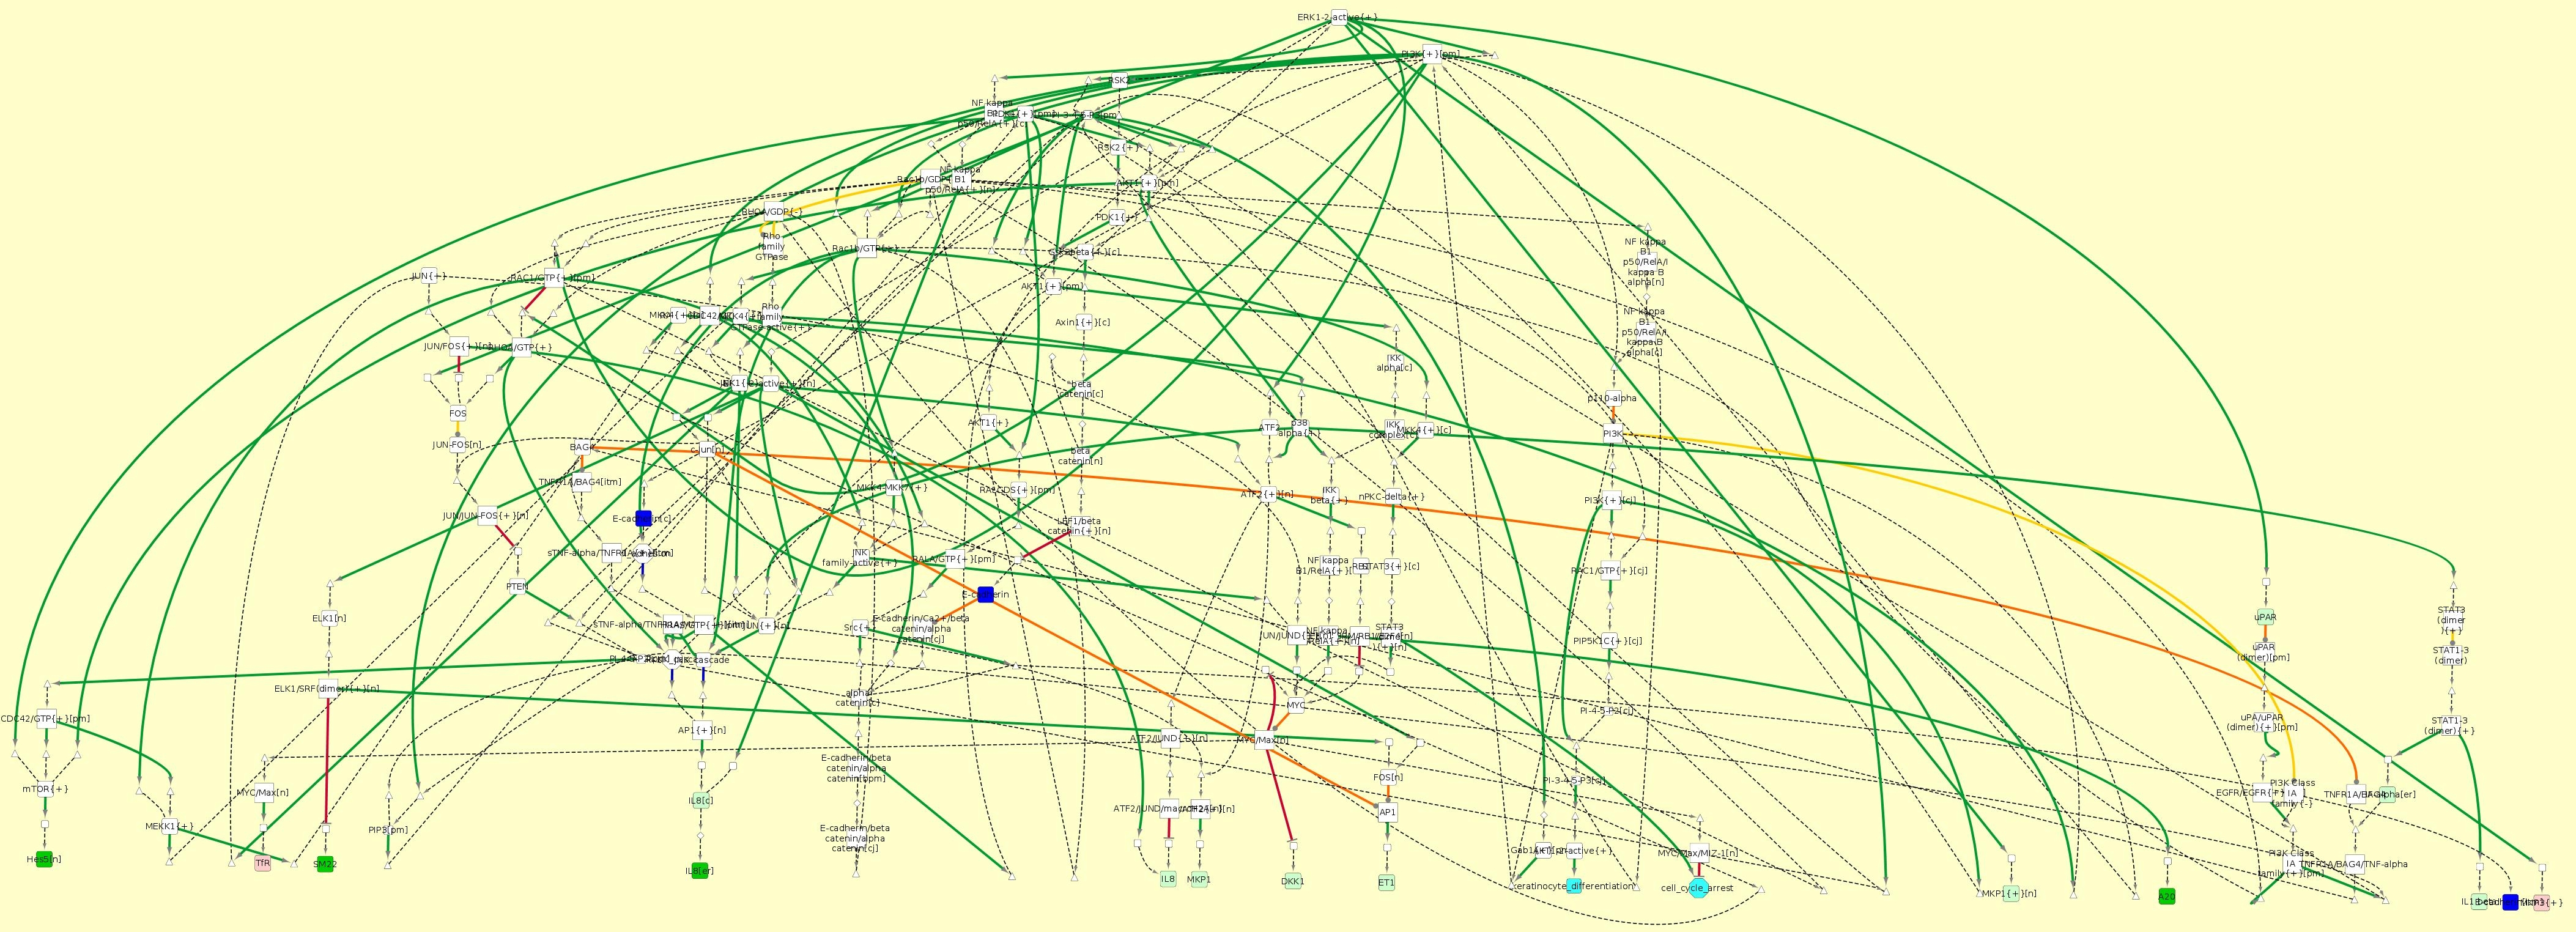
\includegraphics[width=13cm]{net.jpg}
\caption{{\bf RSTC network}} 
 \label{fig:network}
\end{figure}


\section{Results}


\subsection{Modeling the RSTC network as a PH model}

%In this section, we present the modelisation of biological network express with the biochemical reactions in PID. In the following, we will
%present how to transform biological pattern to the PH model. After that, we propose a way of estimating temporal and stochastic
%parameters for the process hitting model. This section will end by the generation of the PH code generation for the simulation.

%\paragraph{Modeling biological patterns to PH model}

%Here is the first and the most important part of this work. 
In order to model the RSTC network \textbf{with a PH model} we selected known biological regulatory patterns (atomic set of biological components and their interacting roles), represented 
as biochemical reactions in the RSTC network, and proposed their PH representation. 
\textbf{For instance} a molecule $a$ that cooperates with a molecule $b$ to activate a molecule $c$\textbf{,} \pref{fig:runningPH} (left), is a regulatory pattern because it is a protein-complex biochemical reaction that appears recurrent times.  
We model this pattern by four sorts \pref{fig:runningPH} (right) $a$, $b$, $c$ and $ab$. Sorts $a$, $b$ and $c$
represent components $a$, $b$ and $c$. We introduce the cooperative sort $ab$ to \textbf{characterize} constraints on components $a$ and $b$.
In our RSTC network, we found $11$ regulatory patterns (see Appendix \ref{annexe1}). 



\subsection{Integrating time-series gene expression data}


\subsubsection{Discretizing times-series data}

Because PH simulation is discrete we need to discretize continuous experimental data, so we can compare our simulation outputs.
The goal of this method was to better determine, according to the gene expression level, when  a given molecule is activated or inhibited.
To do this, we introduced the new analog concept of Significant Increase or Decrease to characterize the fact that a level of a molecule 
increases or decreases when crossing a threshold of significance; \textbf{We} limited the possible expression levels for a molecule to
$\{0, 1, 2\}$. Algorithm \ref{alg:Discretization} underlines the main steps of the proposed discretization method.
\begin{algorithm}
\caption{Discretization of experimental data}
\label{alg:Discretization}
\begin{algorithmic}
\REQUIRE $X$ a table of experimental data
\ENSURE $Y$ a table of discretized data
%\STATE $y \leftarrow initialState(x)$
\FORALL{ gene $i$ in $X$ } 

\STATE $threshold \leftarrow computeThreshold(X[i,]);$
\STATE $Y[i,0] \leftarrow initialState(threshold,X[i,]);$
\FORALL {$j$ in $numberExpression$}
  \IF{$Increase(X[i,j],X[i,j+1])$}
   \STATE $computeSignificativityOfIncrease(threshold,X[i,j],X[i,j+1]);$
   \STATE $\textbf{fixSTATE}(Y[i,j],Y[i,j+1]);$
  \ELSE
   \STATE $computeSignificativityOfDecrease(threshold,X[i,j],X[i,j+1]);$
   \STATE $\textbf{fixSTATE}(Y[i,j],Y[i,j+1]);$
  \ENDIF
\ENDFOR

\ENDFOR

\end{algorithmic}
\end{algorithm}

To illustrate the result of the discretization algorithm \ref{alg:Discretization} we plot in \pref{fig:illustrationDiscretisation} the expression 
of the TFRC and IL8 genes from the times-series data with their respective discrete plots. 
On the discrete plot, one can clearly differentiate when a molecule is active or not, which is of extreme importance 
when modeling these steps in the PH framework \textbf{since we want to have} coherent simulation results.

\begin{figure}
 \centering
 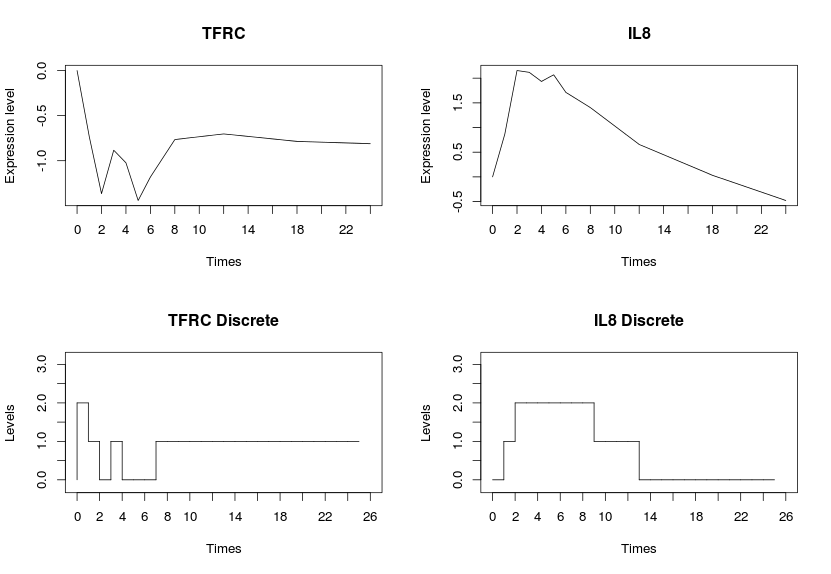
\includegraphics[scale=0.3]{IllustrationDiscretisation.png}
 % IllustrationDiscretisation.png: 831x574 pixel, 72dpi, 29.32x20.25 cm, bb=0 0 831 574
 \caption{Illustration of discretisation of Experiment Data }
 \label{fig:illustrationDiscretisation}
\end{figure}



\subsubsection{Estimating the parameters for the PH-simulation}

The simulation of the execution of the PH actions is done stochastically.  Therefore, we need to relate each action with temporal 
and stochastic parameters, introduced into the PH framework to achieve dynamic refinement \cite{PMR10-TCSB}. 
This is an important aspect of the modeling when taking into account the temporal and stochastic dimensions of 
biological reactions by performing simulations. 
On the one hand, we consider the probability of a reaction to occur, and on the other hand, we 
consider stochastic parameters in the aim at observing an expected behavior. 
In the PH framework, to play an action we need two essential parameters: the rate $r$ or the temporal parameter because $t=r^{-1}$ 
and the stochasticity absorption $sa$. These two parameters will be estimated according to the expression profile of time series data of the experiment. 
To avoid overfitting in the estimation of these parameters, we propose that each component of the PH, representing a measured gene in the network,  will take the estimated values of the parameters of its respective cluster in the experimental data.

\begin{enumerate}
 \item The first step is to cluster the data set. The goal of the clustering process is \textbf{to partition the genes} into groups such that the 
 profiles contained in the same group (cluster) are similar to each other and as different as possible \textbf{of the profiles} assigned to the other
 clusters. The particularity here is to choose the best clustering criteria.
 \item For each cluster obtained in the previous step, estimate the value of $r$ and $sa$ associated to the cluster.
 \item For each component of the PH model associated to the measured gene, determine its cluster, and \textbf{assign it the previously  estimated  parameters}, $r$ and $sa$.
\end{enumerate}

In our time-series data\textbf{,} the components of the PH which need to be associated specific parameters (step 3) are the $12$ genes present in our RSTC network.


\subsection{PH code generation}

To simulate of the model, we generated a PINT code to be simulated by the PINT simulator\footnote{Available at \url{http://process.hitting.free.fr}}. For the PINT code 
generation we first list all the selected patterns in the biological reaction into a file. In this file, each line contains the 
name of the nodes belonging to the current reaction and the reaction type number. The list was then parsed, line by line and, 
after renaming the nodes using numbers (for readability and in conformity with the PINT language syntax) the corresponding PINT code
for the PH process equivalent to each reaction was generated. \textbf{This was implemented in the Java programming language}.


\section{Conclusions}
This work describes the preliminary steps towards the integration of time-series data in large-scale cell-based models. 
We proposed a semi-automatic method to build a PH from a biological system composed of biochemical reactions, extracted \textbf{automatically} from public databases, 
relevant to keratinocyte stimulation induced by \textbf{calcium}. 
We then proposed a method to discretize time-series gene expression data, so they can be confronted to the PH simulations and logically explained by the PH static \textbf{analysis}. 
Finally we described a method to automatically estimate the temporal and stochastic
parameters for the PH simulation, so this estimation process will not be biased by overfitting.
As concrete perspectives of this work, we intend to \emph{(i)} validate the RSTC network topology by confronting its \emph{in-silico} simulation with real measurements of its components;
\emph{(ii)} compare the stochastic simulation results with reachability static analysis over the same PH components mapped to the 12 measured genes; and 
finally \emph{(iii)} search for key-regulators up-stream the 12 genes which will control the dynamics of the system, to  provide our \textbf{biologist  partners} concrete 
hypotheses to test experimentally.

%\paragraph{Acknowledgment}
%This work was partially supported by the region Pays de la Loire.

%\bibliographystyle{plain}
%\bibliography{biblio.bib}

\begin{thebibliography}{10}

\bibitem{batt2005validation}
Gr{\'e}gory Batt, Delphine Ropers, Hidde De~Jong, Johannes Geiselmann, Radu
  Mateescu, Michel Page, and Dominique Schneider.
\newblock Validation of qualitative models of genetic regulatory networks by
  model checking: Analysis of the nutritional stress response in escherichia
  coli.
\newblock {\em Bioinformatics}, 21(suppl 1):i19--i28, 2005.

\bibitem{guziolowski2012automatic}
Carito Guziolowski, Aristotelis Kittas, Florian Dittmann, and Niels Grabe.
\newblock Automatic generation of causal networks linking growth factor stimuli
  to functional cell state changes.
\newblock {\em FEBS Journal}, 279(18):3462--3474, 2012.

\bibitem{guziolowski2013exhaustively}
Carito Guziolowski, Santiago Videla, Federica Eduati, Sven Thiele, Thomas
  Cokelaer, Anne Siegel, and Julio Saez-Rodriguez.
\newblock Exhaustively characterizing feasible logic models of a signaling
  network using answer set programming.
\newblock {\em Bioinformatics}, 29(18):2320--2326, 2013.

\bibitem{macnamara2012state}
Aidan MacNamara, Camille Terfve, David Henriques, Beatriz~Pe{\~n}alver
  Bernab{\'e}, and Julio Saez-Rodriguez.
\newblock State--time spectrum of signal transduction logic models.
\newblock {\em Physical Biology}, 9(4):045003, 2012.

\bibitem{mitsos2009identifying}
Alexander Mitsos, Ioannis~N Melas, Paraskeuas Siminelakis, Aikaterini~D
  Chairakaki, Julio Saez-Rodriguez, and Leonidas~G Alexopoulos.
\newblock Identifying drug effects via pathway alterations using an integer
  linear programming optimization formulation on phosphoproteomic data.
\newblock {\em PLoS computational biology}, 5(12):e1000591, 2009.

\bibitem{mobashir2012simulated}
Mohammad Mobashir, Burkhart Schraven, and Tilo Beyer.
\newblock Simulated evolution of signal transduction networks.
\newblock {\em PloS one}, 7(12):e50905, 2012.

\bibitem{PMR10-TCSB}
{L}o{\"i}c {P}aulev{\'e}, {M}organ {M}agnin, and {O}livier {R}oux.
\newblock Refining dynamics of gene regulatory networks in a stochastic
  $\pi$-calculus framework.
\newblock In {\em Transactions on Computational Systems Biology XIII}, pages
  171--191. Springer, 2011.

\bibitem{schaefer2009pid}
Carl~F Schaefer, Kira Anthony, Shiva Krupa, Jeffrey Buchoff, Matthew Day, Timo
  Hannay, and Kenneth~H Buetow.
\newblock Pid: the pathway interaction database.
\newblock {\em Nucleic acids research}, 37(suppl 1):D674--D679, 2009.

\bibitem{tyson2003sniffers}
John~J Tyson, Katherine~C Chen, and Bela Novak.
\newblock Sniffers, buzzers, toggles and blinkers: dynamics of regulatory and
  signaling pathways in the cell.
\newblock {\em Current opinion in cell biology}, 15(2):221--231, 2003.

\bibitem{yu2012hipathdb}
Namhee Yu, Jihae Seo, Kyoohyoung Rho, Yeongjun Jang, Jinah Park, Wan~Kyu Kim,
  and Sanghyuk Lee.
\newblock hipathdb: a human-integrated pathway database with facile
  visualization.
\newblock {\em Nucleic acids research}, 40(D1):D797--D802, 2012.

\end{thebibliography}



%\appendix

\clearpage
\appendix
\section*{Appendix A}
\label{annexe1}
% ...
\begin{figure}[ht]
\begin{tabular}{|c|c|}
\hline
Biological Pattern no $1$ & PH Model \\
\hline
 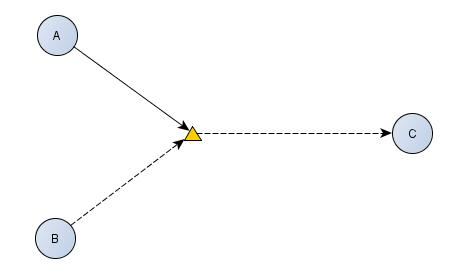
\includegraphics[scale=0.3]{./imagesannexe/phdrawings/1cyt.jpg} & 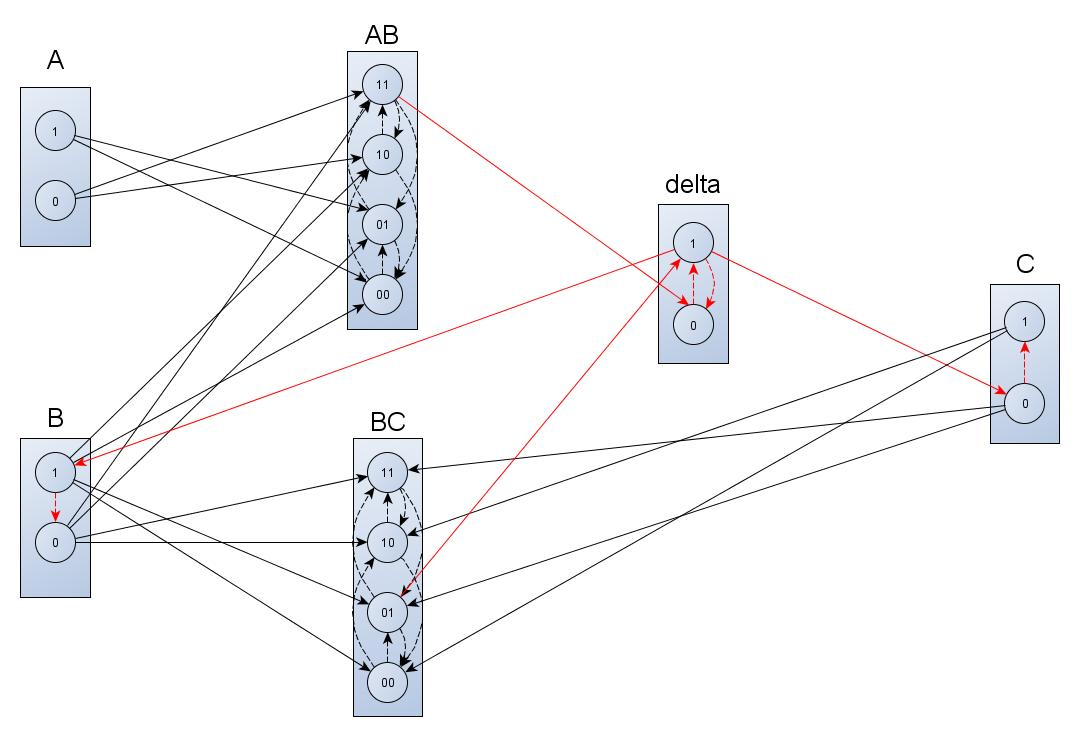
\includegraphics[scale=0.15]{./imagesannexe/phdrawings/1ph.jpg} \\
 \hline
\end{tabular}
\caption{\label{fig:pattern:1}
(left)~Biological pattern: Molecules A and B cooperate to activate molecule C. After the activation of C, A remains 
active and B is desactivated.
(right)~equivalent PH model. AB and BC are regular sorts, while the sort delta models the reaction beginning or end.
}
\end{figure}

\begin{figure}[ht]
\begin{tabular}{|c|c|}
\hline
Biological Pattern no $2$ & PH Model \\
\hline
  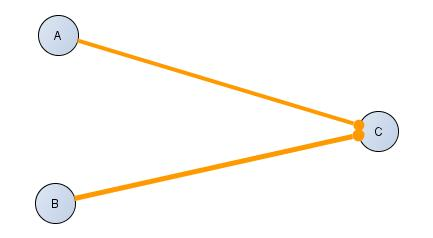
\includegraphics[scale=0.3]{./imagesannexe/phdrawings/2cyt.jpg} & 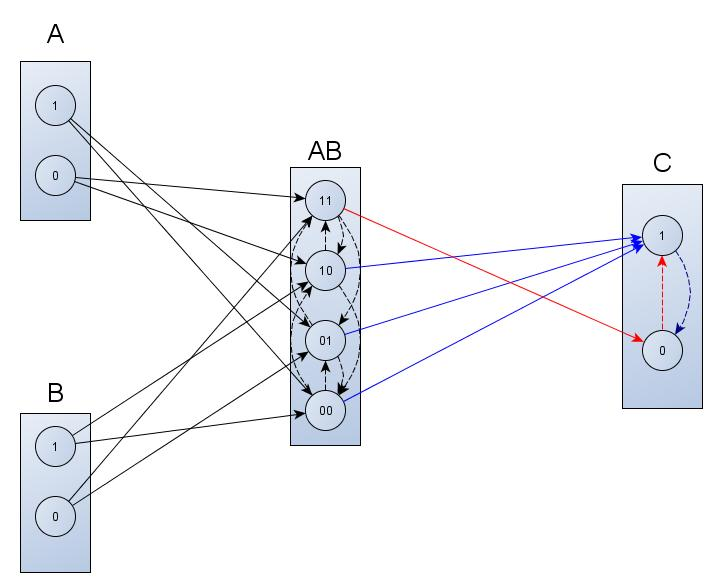
\includegraphics[scale=0.15]{./imagesannexe/phdrawings/2ph.jpg} \\
 \hline
 
\end{tabular}
\caption{\label{fig:pattern:2}
(left)~Biological pattern: A and B cooperate to activate C. Both A and B remain active after end of reaction
(right)~equivalent PH model
}
\end{figure}

\begin{figure}[ht]
\begin{tabular}{|c|c|}
\hline
Biological Pattern no $3$ & PH Model \\
\hline
 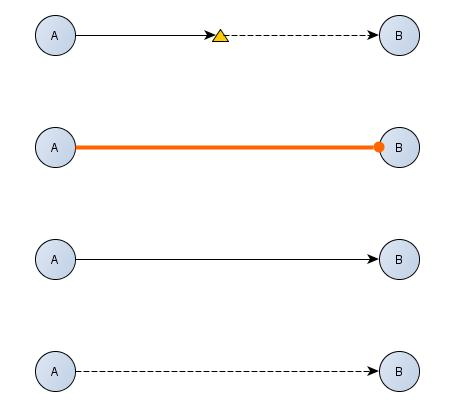
\includegraphics[scale=0.3]{./imagesannexe/phdrawings/3cyt.jpg} & 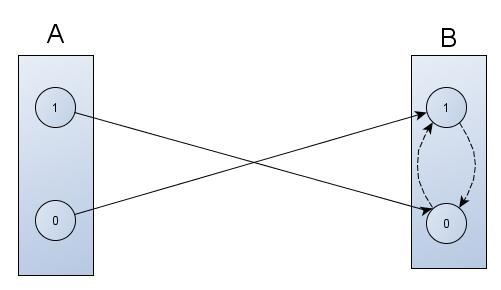
\includegraphics[scale=0.15]{./imagesannexe/phdrawings/3ph.jpg} \\
 \hline
\end{tabular}
\caption{\label{fig:pattern:3}
(left)~Biological pattern: different types of activation.
(right)~equivalent PH model
}
\end{figure}

\begin{figure}[ht]
\begin{tabular}{|c|c|}
\hline
Biological Pattern no $4$ & PH Model \\
\hline
 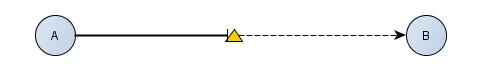
\includegraphics[scale=0.3]{./imagesannexe/phdrawings/4cyt.jpg} & 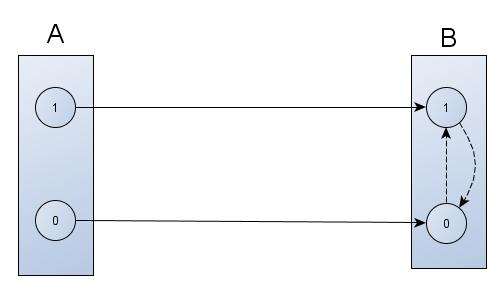
\includegraphics[scale=0.14]{./imagesannexe/phdrawings/4ph.jpg} \\
 \hline
\end{tabular}
\caption{\label{fig:pattern:4}
(left)~Biological pattern of an inhibition reaction: the inhibitor presence leads to the desactivation of its target,
while its absence leads to the activation of the target
(right)~equivalent PH model
}
\end{figure}

\begin{figure}[ht]
\begin{tabular}{|c|c|}
\hline
Biological Pattern no $5$ & PH Model \\
\hline
 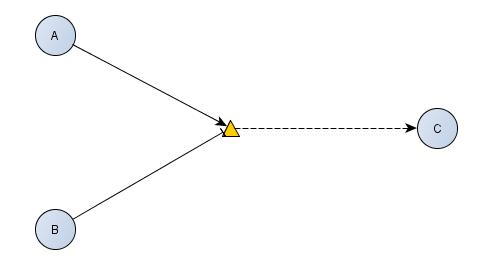
\includegraphics[scale=0.3]{./imagesannexe/phdrawings/5cyt.jpg} & 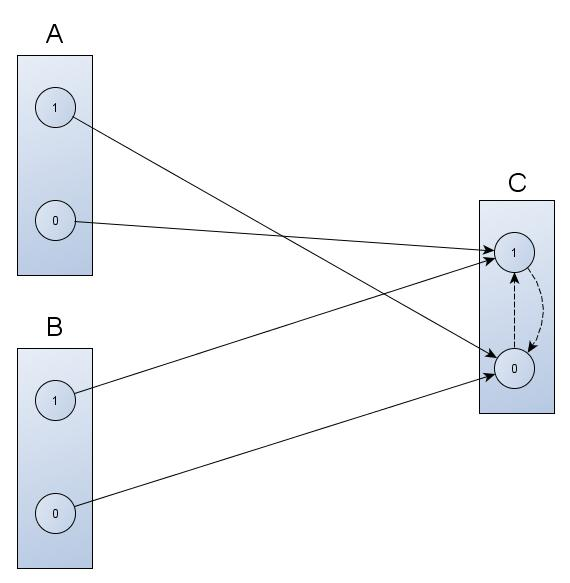
\includegraphics[scale=0.14]{./imagesannexe/phdrawings/5ph.jpg} \\
 \hline
\end{tabular}
\caption{\label{fig:pattern:5}
(left)~Biological pattern. Molecule C is either activated by A, or inhibited by B;
(right)~equivalent PH model where A and B are not cooperating to modify C, each one has independent, opposite action on C.
}
\end{figure}

\begin{figure}[ht]
\begin{tabular}{|c|c|}
\hline
Biological Pattern no $6$ & PH Model \\
\hline
 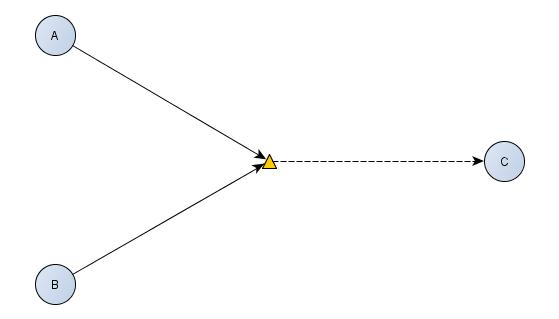
\includegraphics[scale=0.25]{./imagesannexe/phdrawings/6cyt.jpg} & 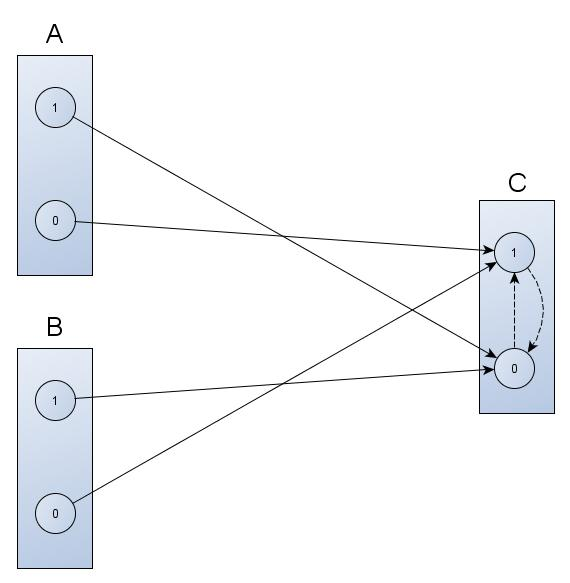
\includegraphics[scale=0.15]{./imagesannexe/phdrawings/6ph.jpg} \\
 \hline
\end{tabular}
\caption{\label{fig:pattern:6}
(left)~ Molecule C is activated by either A, or B, independantly one from other.
(right)~equivalent PH model
}
\end{figure}

\begin{figure}[ht]
\begin{tabular}{|c|c|}
\hline
Biological Pattern no $7$ & PH Model \\
\hline
  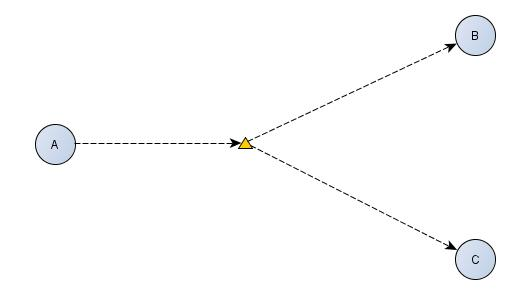
\includegraphics[scale=0.3]{./imagesannexe/phdrawings/7cyt.jpg} & 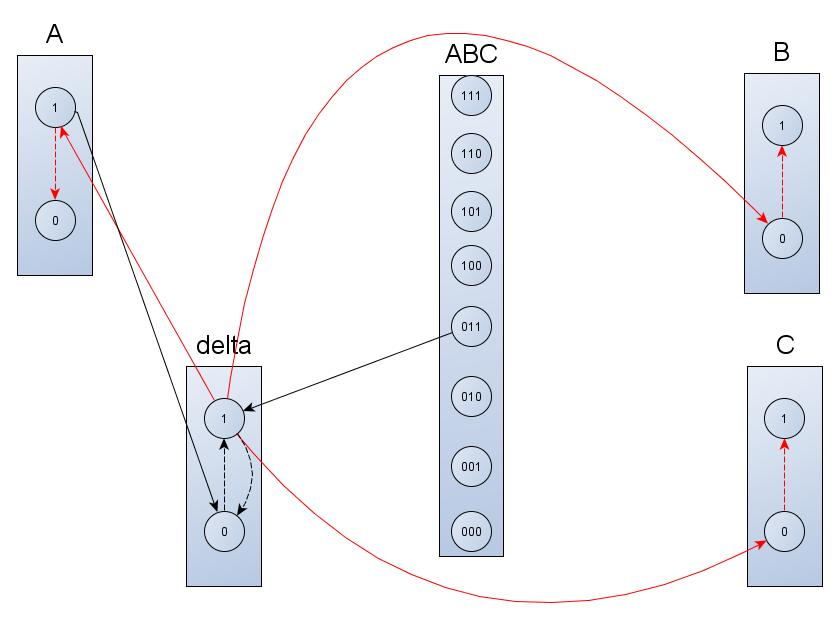
\includegraphics[scale=0.15]{./imagesannexe/phdrawings/7ph.jpg} \\
 \hline
\end{tabular}
\caption{\label{fig:pattern:7}
(left)~ Complex A decomposes in components B and C. At the end of the reaction, A no longer exists/ is no
longer active.
(right)~equivalent PH model. ABC is a regular cooperative sort and delta models the reaction,
as explained in Pattern 1. For clarity purposes, the hits from A, B and C to the cooperative
sort ABC have not been drawn.
}
\end{figure}

\begin{figure}[ht]
\begin{tabular}{|c|c|}
\hline
Biological Pattern no $8$ & PH Model \\
\hline
 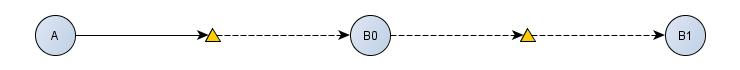
\includegraphics[scale=0.3]{./imagesannexe/phdrawings/8cyt.jpg} & 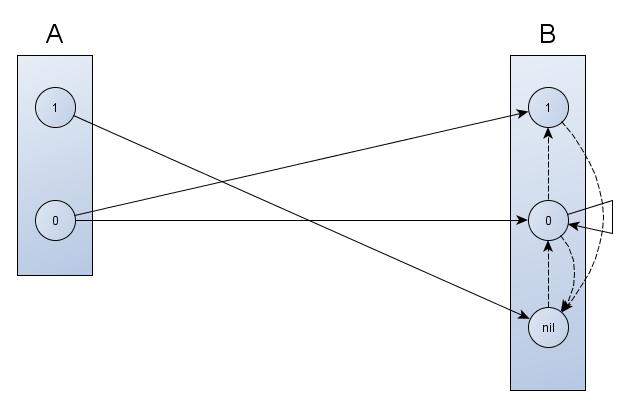
\includegraphics[scale=0.12]{./imagesannexe/phdrawings/8ph.jpg} \\
 \hline
\end{tabular}
\caption{\label{fig:pattern:8}
(left)~ $B0$ and $B1$ represent the same biological entity.
(right)~equivalent PH model, $B0$ and $B1$ are different process of the same sort; A create B, which then activates itself.
}
\end{figure}

\begin{figure}[ht]
\begin{tabular}{|c|c|}
\hline
Biological Pattern no $9$ & PH Model \\
\hline
 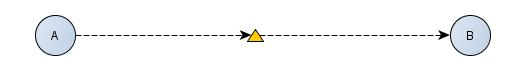
\includegraphics[scale=0.3]{./imagesannexe/phdrawings/9cyt.jpg} & 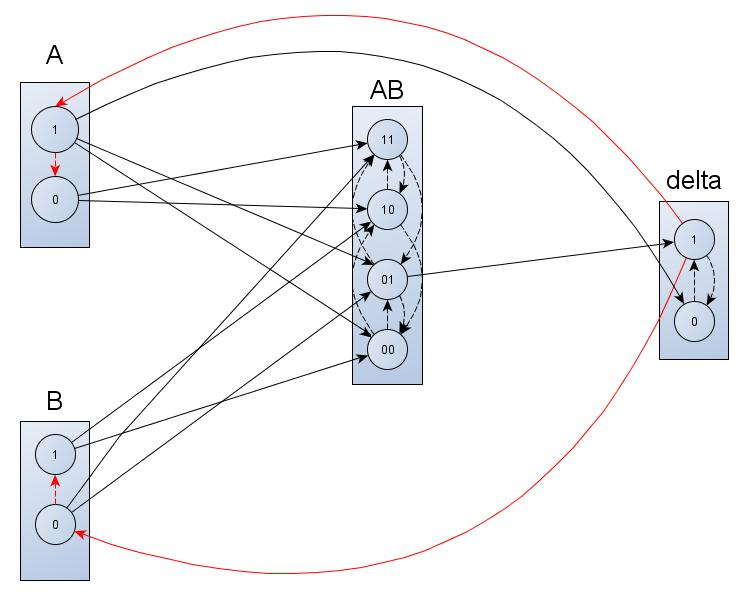
\includegraphics[scale=0.12]{./imagesannexe/phdrawings/9ph.jpg} \\
 \hline
\end{tabular}
\caption{\label{fig:pattern:9}
(left)~A modification reaction: A activate B, then dissapears; The reaction begins when A is present, and ends when A has replaced by B.
(right)~equivalent PH model, AB is a cooperative sort and the delta sort models the reaction.
}
\end{figure}

\begin{figure}[ht]
\begin{tabular}{|c|c|}
\hline
Biological Pattern no $10$ & PH Model \\
\hline
 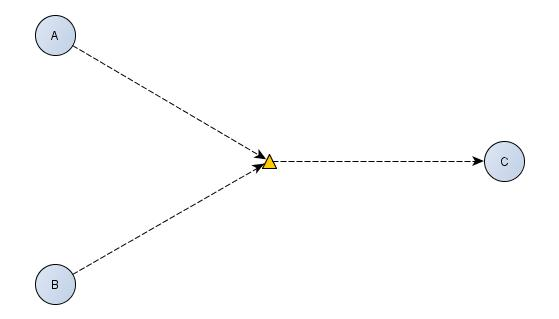
\includegraphics[scale=0.3]{./imagesannexe/phdrawings/10cyt.jpg} & 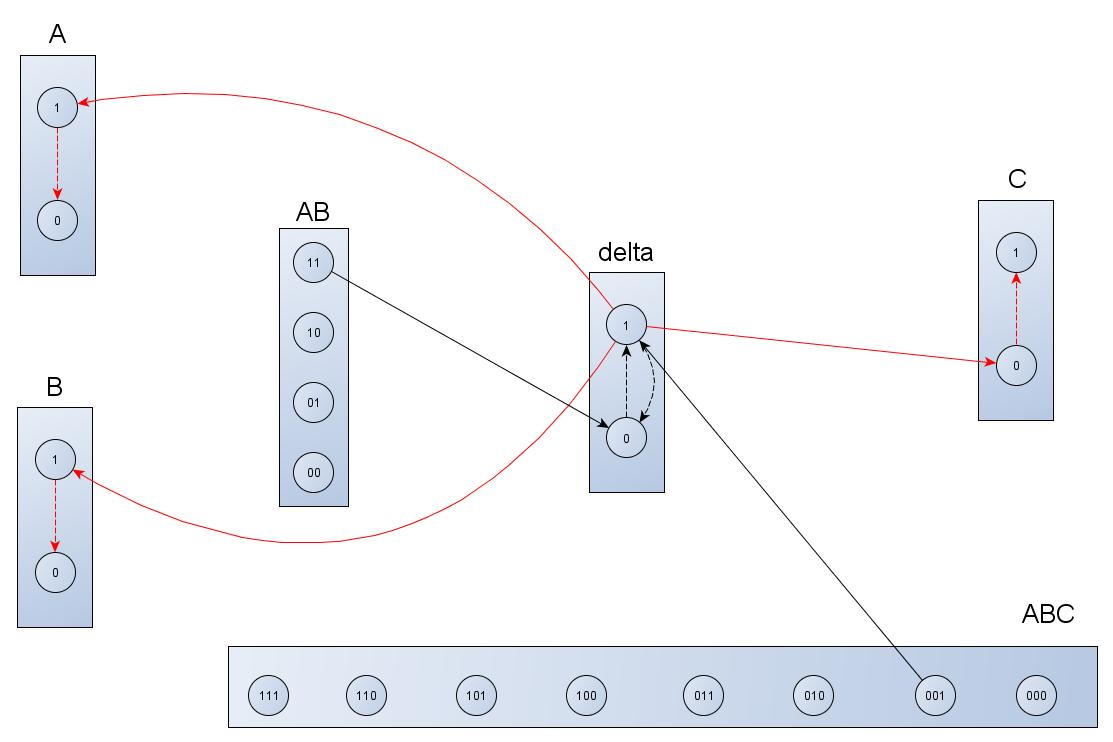
\includegraphics[scale=0.15]{./imagesannexe/phdrawings/10ph.jpg} \\
  \hline
\end{tabular}
\caption{\label{fig:pattern:10}
(left)~A composite modification: A and B cooperate to create C, then disappear. 
(right)~equivalent PH model. For clarity purposes, 
hits to cooperative sorts have not been drawn.
}
\end{figure}

\begin{figure}[ht]
\begin{tabular}{|c|c|}
\hline
Biological Pattern no $11$ & PH Model \\
\hline
  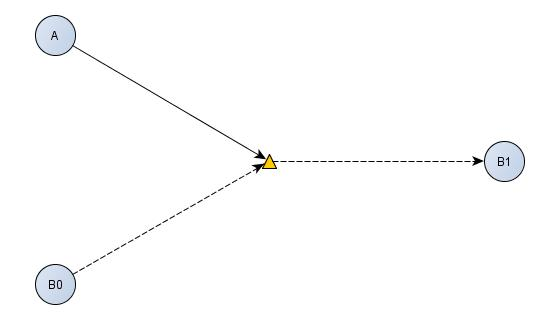
\includegraphics[scale=0.28]{./imagesannexe/phdrawings/11cyt.jpg} & 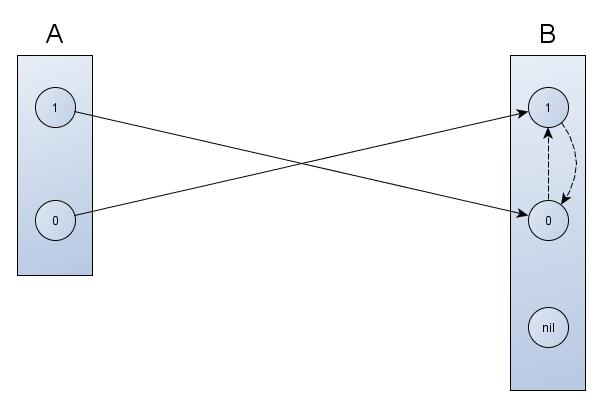
\includegraphics[scale=0.15]{./imagesannexe/phdrawings/11ph.jpg} \\
 \hline
\end{tabular}
\caption{\label{fig:pattern:11}
(left)~Activation of non-binary sort: similar to Pattern $1$, except for the non-binarity of the target source.
$B0$ and $B1$ represent the same entity. Unlike pattern $8$ (the other pattern dealing with non-binary sorts),
entity B is already present, via the condition on $B0$, it just needs to be activates.
(right)~equivalent PH model. 
}
\end{figure}



\clearpage
\section*{Appendix B}
\label{annexe2}
\begin{figure}[ht]
\newcolumntype{M}[1]{>{\raggedright}m{#1}}
\begin{tabular}{|l|M{4cm}|}
\hline
Functions  & Specifications \tabularnewline
\hline
 computeThreshold(X) &  compute the threshold of the profile of expression represent by X \tabularnewline
 \hline
 initialState(X) & fixe the initial state of the expression represent by X according to the initial value of X and the threshold \tabularnewline 
 \hline
 Increase(X,Y) & Test if the measure increases between the two times points X and Y \tabularnewline 
 \hline
 computeSignificativityOfIncrease(s,X1,X2) & compute the significance of the increase according to the threshold and X1 and X2 \tabularnewline
 \hline
 computeSignificativityOfDecrease(s,X1,X2) & compute the significance of the decrease according to the threshold and X1 and X2 \tabularnewline
 \hline
 fixSTATE(X1, X2) & fix the current state  \tabularnewline
  \hline
\end{tabular}
\caption{\label{fig:specification of functions used in the algorithm}
Functions(first column) and Specifications(second column)
}
\end{figure}


\clearpage
\section*{Appendix C}
\begin{figure}[hb]
 \centering
 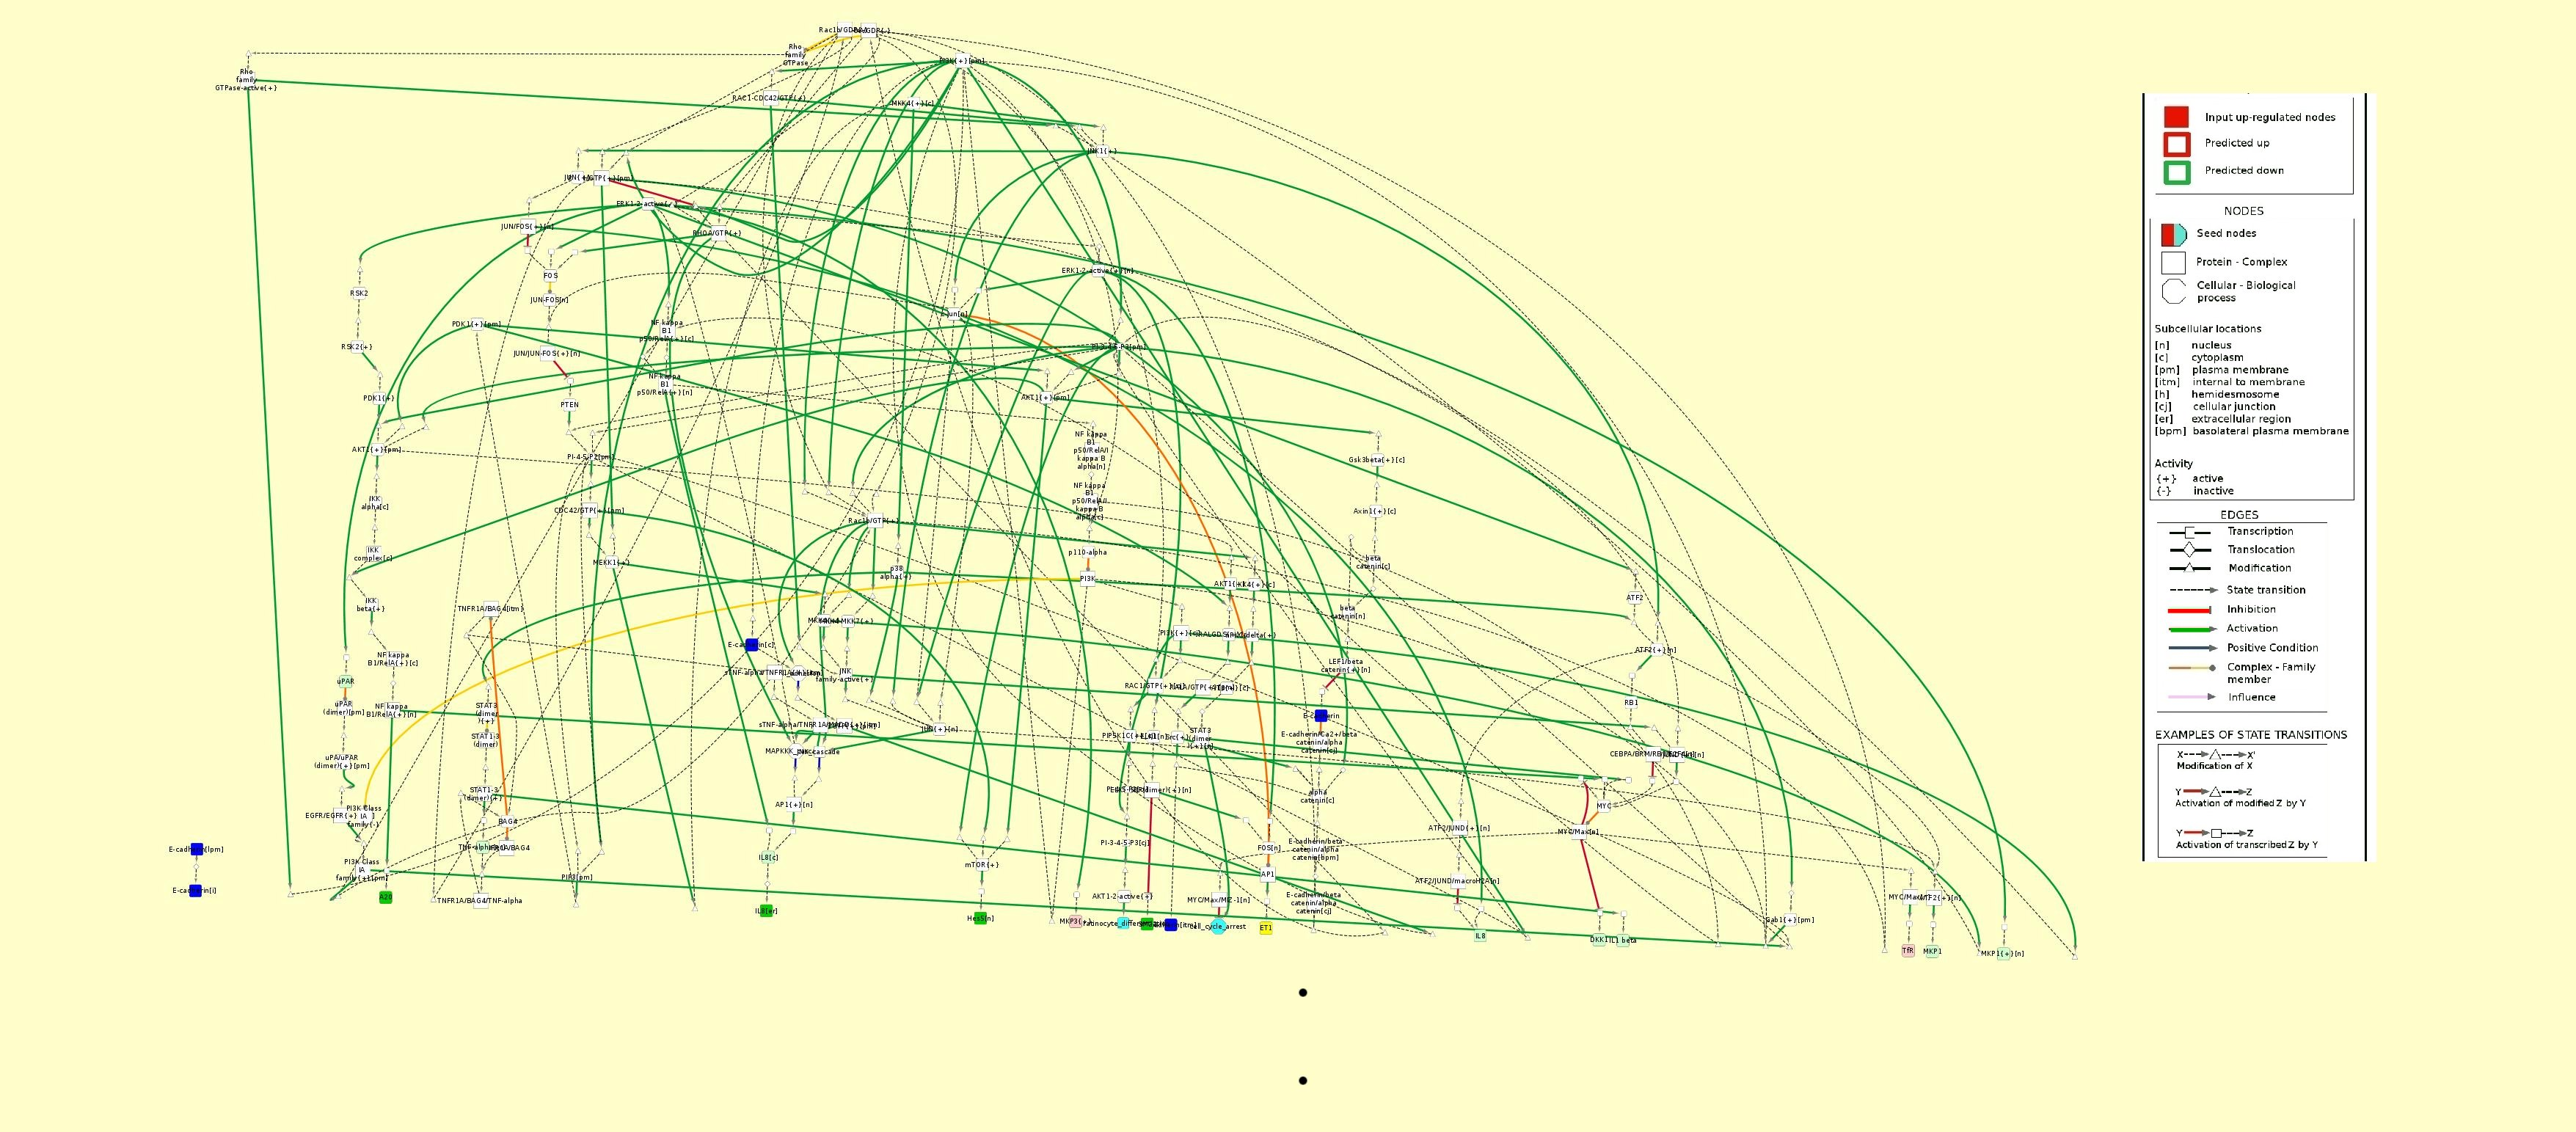
\includegraphics[angle=270, scale=0.12,clip=true,trim=165pt 12pt 200pt 12pt]{./RstcbiologicalNetwork3.jpeg}
 % RstcbiologicalNetwork3.jpeg: 3511x1543 pixel, 72dpi, 123.86x54.43 cm, bb=0 0 3511 1543
 \caption{RSTC Network}
 \label{fig:RSTCNetwork}
\end{figure}


\end{document}
